%-------------------------------------------------------------------------------
%   Haskellerのための圏論
%   Keichi
%   圏論の勉強成果の個人的なまとめ
%-------------------------------------------------------------------------------

\documentclass{jsarticle}

%各種パッケージを読み込む
%ソースコードフォーマット・強調表示
\usepackage{listings,jlisting}
%図の埋め込み
\usepackage[dvipdfm]{graphicx}
%URLの埋め込み
\usepackage{url}

%ソースコードの表示のデフォルトフォーマットを設定
\lstset{
    %言語
    language={Haskell},
    basicstyle={\small},
    %識別子のスタイル
    identifierstyle={\small},
    %コメントの書体
    commentstyle={\small\itshape},
    %キーワードの書体
    keywordstyle={\small\bfseries},
    ndkeywordstyle={\small},
    %文字列リテラルの書体
    stringstyle={\small\ttfamily},
    frame={htbp},
    %行が長くなったときの改行
    breaklines=true,
    columns=[l]{fullflexible},
    %行番号の表示
    %numbers=left,
    xrightmargin=0zw,
    xleftmargin=3zw,
    numberstyle={\scriptsize},
    stepnumber=1,
    numbersep=1zw,
    lineskip=-0.5ex
}


%-------------------------------------------------------------------------------
\begin{document}

\title{Haskellerのための圏論}
\author{Keichi}
\maketitle

\section{はじめに}
この文書はHaskellを勉強している筆者が、寄り道して勉強した圏論について、
学習した事項をまとめたものです。主な内容は、HaskellWikiのCategory theoryの
ページ\cite{wiki}の翻訳です。
この文書は、Wikiの内容にHaskellで書いたサンプルコードや、図、用語の解説などを
多少書き加えたものです。

Haskellは、圏論をプログラミング言語に応用してつくられた言語です。
ただし圏論を知らなくても、Haskellの概念を理解することはできますし、
コード自体は書けます。ただしファンクタやモナドなどの概念を考えた側は、
圏論から着想を得ているわけで、圏論を学ぶことでより深くHaskellを理解できると
私は思っています。

%-------------------------------------------------------------------------------
\section{圏}

\subsection{定義}
ある圏(Category)$C$は、2つの集合の組からなる:

\begin{itemize}
    \item $Ob(C)$、$C$の「対象」(Object)の集合
    \item $Ar(C)$、$C$の「射」(Morphism)の集合
\end{itemize}

$Ar(C)$に含まれる射$f$は、$Ob(C)$の要素であるドメイン(Domain)
(もしくはソース(Source))$dom f$と、コドメイン(Codomain)(もしくはターゲット(Target))
$cod f$を持つ。$f:A \to B$と書けば、fのドメインが$A$であり、コドメインが
$B$であることを意味する。

\begin{figure}[htbp]
    \centering
    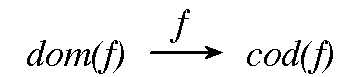
\includegraphics{diag_dom.pdf}
    \caption{ドメインとコドメイン}
\end{figure}

また合成という操作が存在し、これは$\circ$と表記される。
例えば、射$g \circ f$が定義されるとき、$f$のコドメインは$g$のドメインと等しく、
$g \circ f$のドメインとコドメインはそれぞれ$f$のドメインと$g$のコドメイン
となる。つまり、射$f$と$g$が存在し、$f:A \to B$かつ$g:B \to C$ならば、
$g \circ f = A \to C$ということである。また、ある対象$A$について、
$id_A: A \to A$という射が定義される。これは恒等射と呼ばれ、
$id$とだけ表記されることも多い。

\begin{figure}[htbp]
    \centering
    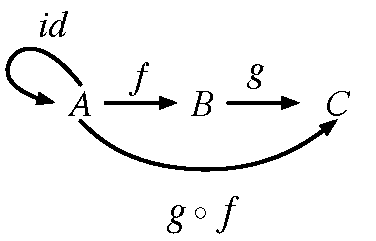
\includegraphics{diag_comp.pdf}
    \caption{恒等射と合成}
\end{figure}

また、圏$C$においてHomset集合を
$hom_C(A,B)=\{f \mid f \in Ar(C), f: A \to B\}$と定義する。
これはつまり、圏$C$において対象$A$から$B$への射の集合である。

\subsection{公理}
また、$C$が圏であるためには、以下の条件が満たされている必要がある:
\begin{itemize}
    \item $f:A \to B$なら$f \circ id_A = id_b \circ f = f$
        (恒等射は左単位元、右単位元である)
    \item $f:A \to B$かつ$g: B \to C$か$h: B \to D$なら、
        $h \circ (g \circ f)=(h\circ g) \circ f$(射は結合律を満たす)
\end{itemize}

\subsection{圏の例}
\begin{itemize}
    \item Set, 集合を対象とし、集合間の写像を射とする
    \item Mon, モノイドを対象とし、モノイドの射を射とする
        (モノイドは対象が1つだけの圏ともとらえれる)
    \item Grp, 群を対象とし、群の準同型写像を射とする
    \item Hask, Haskellの型を対象とし、関数を射とする圏
    \item Cat, 圏を対象とし、関手を射とする圏の圏
    \item 関数を対象とし、データの流れを射とする圏(データフローダイアグラム)
\end{itemize}

\subsection{Haskellでの例}
Haskellの型と関数からなる圏Haskを考えると、
圏Haskの対象$Ob(Hask)$は全てのHaskellの型の集合、
\[\{Int, Bool, Float, String, \ldots\}\]
である。また、$Ar(Hask)$は全てのHaskellの関数の集合、
\[\{(+), length, even, \ldots\}\]
となる。圏Haskにおいて射の合成$\circ$は、関数合成演算子
\begin{lstlisting}
    (.)::(b->c)->(a->b)->(a->c)
\end{lstlisting}
であり、恒等射は恒等関数
\begin{lstlisting}
   id::a->a
\end{lstlisting}
となる。単位元律および結合律が成り立つのは明らかである。(seqなどの例外はあるが)

%-------------------------------------------------------------------------------
\newpage
\section{関手}

\subsection{定義}
$C$, $D$を圏とすると、関手(Functor)$F:C \to D$は
関数$F_{objects}:Ob(C) \to Ob(D)$と関数$F_{arrows}:Ar(C)\to Ar(D)$の組である。
前者は対象関数とよばれ、後者は射関数とよばれる。

\begin{figure}[htbp]
    \centering
    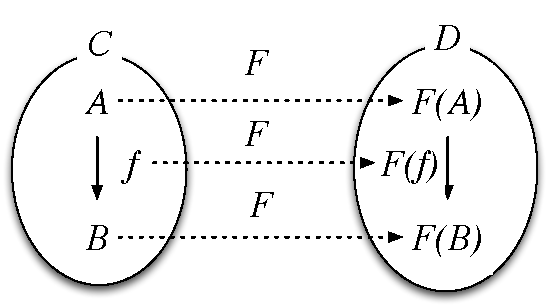
\includegraphics{diag_functor.pdf}
    \caption{関手$F$}
\end{figure}

\subsection{公理}
\begin{itemize}
    \item 圏$C$において$f:A\to B$が存在すれば、
        圏$D$において$F(f):F(A)\to F(B)$である
    \item 圏$C$において$g:B\to C$、$f:A\to B$が存在すれば、
        $F(f)\circ F(g)=F(f\circ g)$が成り立つ
    \item 圏$C$の全ての対象について、$id_{F(A)}=F(id_A)$
\end{itemize}

\subsection{Haskellにおける関手}
厳密には、Haskell圏における関手は、Haskellの型と関数に対するあらゆる操作うち、
上記の公理を満たすものである。しかし、Haskellはプログラミング言語であるので、
実際Haskellで扱うのは、対象関数と射関数の両方がHaskellで書ける関手だけである。
具体的には、Haskellにおける関手の対象関数は、
多くの場合データコンストラクタであり、射関数は多相関数fmapとなる。
これは型クラスFunctorで宣言されている:

\begin{lstlisting}
class Functor f where
    fmap :: (a -> b) -> (f a -> f b)
\end{lstlisting}

Haskellにおいて、ListやMaybe、Treeなどは全てFunctorクラスの
インスタンスであり、Functorクラスのインスタンスは以下の条件
\begin{lstlisting}
    fmap id = id
    fmap f . fmap g = fmap (f . g)
\end{lstlisting}
を満たすべきであるとされている。これは上記の公理に相当する。

具体的な例として、Hask圏からMaybe圏への関手Maybeを考える。
関手Maybeの対象関数はJustであり、射関数はfmapとなる。
\begin{lstlisting}
    --元の圏の上での関数f
    f :: Int -> Int
    f x =  x * x

    --fをMaybeの圏の射に写像する
    g :: Maybe Int -> Maybe Int
    g = fmap f

    --元の圏の上での値
    a = 3
    --aをMaybeの圏の対象に写像する
    b = Just a

    main = do
        --元の圏の上で対象に射を適用
        print $ f a
        --Maybeの圏の上で対象に射を適用
        print $ g b
\end{lstlisting}


%-------------------------------------------------------------------------------
\newpage

\section{自然変換}
\subsection{定義}
$C, D$を圏とし、$\Phi,\Psi:C\to D$を関手、$X,Y\in Ob(C)$とし、
$f\in hom_C(X,Y)$とする。

\begin{figure}[htbp]
    \centering
    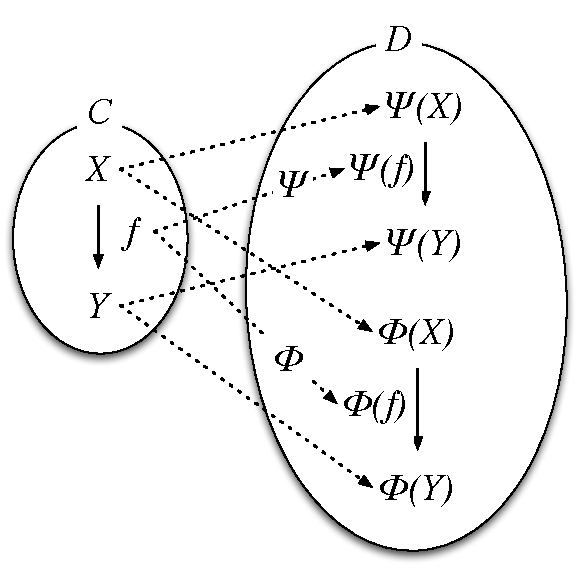
\includegraphics{diag_nt.pdf}
    \caption{関手$\Phi$と$\Psi$}
\end{figure}

自然変換(Natural Transoformation)$\eta:\Phi\to\Psi$は、$C$の各対象を、
以下の条件を満たす$D$の射と対応づける関数である。
\begin{itemize}
    \item $\forall A\in Ob(C)\to \eta_A\in hom_D(\Phi(A),\Psi(A))$
    \item $\eta_Y\circ \Phi(f)=\Psi(f)\circ\eta_X$
\end{itemize}
ここで、$\eta_A$を$A$における$\eta$のコンポーネントとよぶ。
よって、\textbf{$D$において}図\ref{figNatTrans}の関係が成り立つ。

\newpage

\begin{figure}[htbp]
    \centering
    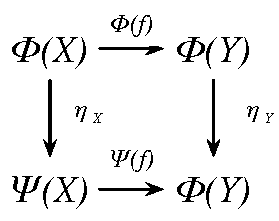
\includegraphics{diag_nt2.pdf}
    \caption{自然変換$\eta$}
    \label{figNatTrans}
\end{figure}

\subsection{Haskellによる例}
これは、図\ref{figNatTrans}関係の具体的な例Haskellで書いたものである。
\begin{lstlisting}
    --この関数はData.Maybeで定義されています。
    maybeToList :: Maybe a -> [a]
    maybeToList Nothing     =   []
    maybeToList (Just a)    =   [a]

    main = do
        print $ fmap even $ maybeToList $ Just 5
        print $ maybeToList $ fmap even $ Just 5
\end{lstlisting}
この例と上の図\ref{figNatTrans}の対応関係を考えてみる。
ファンクタ$\Psi$はList、ファンクタ$\Phi$はMaybeと対応する。
また、自然変換$\eta_X$、$\eta_Y$はmaybeToListに相当する。
(ここでmaybeToListは多相関数であるため、$\eta_X$と$\eta_Y$は
1つの多相関数maybeToListに集約される)また、$f$はevenであり
、これがfmapによってそれぞれ$\Psi(f)$と$\Phi(f)$にリフトされる。
fmapは多相であるため、$\Phi$、$\Psi$両方のファンクタの射部分に対応する。

\newpage
\section{Kleisliトリプル}

\subsection{定義}
Haskellで一般的に「モナド」と呼ばれているものは実は圏論のモナドとは
異なっていって、直接的に対応するのは圏論でKleisliトリプルとよばれている。

圏$C$上のKleisliトリプル(Kleisli-Triple)とは
\begin{itemize}
    \item 関数$T:Ob(C)\to Ob(C)$
    \item 射$\eta_A:\to T(A)$(各$A\in Ob(C)$)
    \item $(-)^*$: 射$f^*:T(A)\to T(B)$を各$f:A\to T(B)\in Ar(C)$についてつくる演算子
\end{itemize}
からなる3つ組(トリプル)$(T, \eta, (-)^*)$である。

\subsection{公理}
また、Kleisliトリプルは以下の条件を満たす:
\begin{itemize}
    \item $\eta_A^*=id_{T(A)}$
    \item $f:A\to T(B)$なら、$f^*\circ \eta_A=f$
    \item $f:A\to T(B)$なら、$g^*\circ f^*=(g^*\circ f)^*$
\end{itemize}

\begin{figure}[htbp]
    \centering
    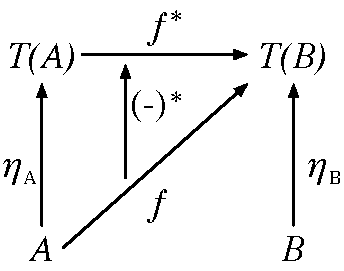
\includegraphics{diag_kleisli.pdf}
    \caption{Kleisliトリプル}
\end{figure}

\subsection{Haskellでの例}
HaskellのモナドはKleisliトリプルと対応する。型クラスMonadの定義は
\begin{lstlisting}
class Monad t where
    (>>=)   ::  t a -> (a -> t b) -> t b
    return  ::  a -> t a
\end{lstlisting}
であり、これはそれぞれ、
\begin{itemize}
    \item Monadのインスタンスのデータコンストラクタ(MaybeならJust)が関数$T$
    \item returnが$\eta$
    \item $(=<<)$が$(-)^*$
\end{itemize}
というように圏論のKleisliトリプルと対応している。
また、上記のKleisliトリプルの満たすべき条件は、以下のHaskellのモナド則に
それぞれ対応する。
\begin{lstlisting}
    (return x) >>= f    == f x
    m >>= return        ==  m
    (m >>= f) >>= g     ==  m >>= (\x -> f x >>= g)
\end{lstlisting}

\begin{thebibliography}{99}

\bibitem{wiki}\url{http://www.haskell.org/haskellwiki/Category_theory}

\end{thebibliography}
\end{document}

